\documentclass[12pt]{article}


\usepackage{amsmath,amssymb,amsthm,enumerate,graphicx}
\usepackage{ifthen,latexsym,syntonly}
\usepackage{setspace}
%\usepackage[showrefs]{refcheck}  %use this to show equation and section labels
\usepackage{color}
\usepackage[round,comma,authoryear]{natbib}   % for natbib
\usepackage{subfigure}
\usepackage{float}
\usepackage{epstopdf}
\usepackage{bm}



\bibliographystyle{mynat}


\onehalfspacing


   % for natbib
%\bibpunct{(}{)}{,}{a}{}{,}  % for natbib
%                            % need to have mynat.bst in an accesssible directory


\bibpunct{(}{)}{,}{a}{}{,}  % for natbib
                            % need to have mynat.bst in an accesssible directory

\newcommand{\EE}{\mathbb E}
\newtheorem{theorem}{Theorem}[section]
\newtheorem{remark}[theorem]{Remark}
\newtheorem{assumption}[theorem]{Assumption}
%\newtheorem{case}[theorem]{Case}
\newtheorem{claim}[theorem]{Claim}
%\newtheorem{conclusion}[theorem]{Conclusion}
\newtheorem{corollary}[theorem]{Corollary}
\newtheorem{condition}[theorem]{Condition}
\newtheorem{criterion}[theorem]{Criterion}
\newtheorem{definition}[theorem]{Definition}
\newtheorem{example}[theorem]{Example}
\newtheorem{lemma}[theorem]{Lemma}
\newtheorem{problem}[theorem]{Problem}
\newtheorem{proposition}[theorem]{Proposition}
%\newtheorem{solution}[theorem]{Solution}
%\newtheorem{summary}[theorem]{Summary}
\newtheorem{thm}[theorem]{Theorem}



\setlength{\oddsidemargin}{.05in} \setlength{\topmargin}{-.45in}
\setlength{\textwidth}{6.4in} \setlength{\textheight}{8.5in}


%\pagestyle{empty}

\title {Optimal Taxation with Incomplete Markets}
%\author{Anmol Bhandari, David Evans, Mikhail Golosov, Thomas J. Sargent}
\author{\textbf{Anmol Bhandari}\\apb296@nyu.edu \and \textbf{David Evans} \\ \texttt{dgevans@nyu.edu} \and \textbf{Mikhail Golosov}\\\texttt{golosov@princeton.edu} \and \textbf{Thomas J. Sargent} \\ \texttt{thomas.sargent@nyu.edu}
}

\begin{document}

\maketitle



\begin{abstract}

\end{abstract}


\noindent\textsc{Keywords:}
\section{Introduction}


\section{Environment}




 Markov aggregate shocks $s_t\in \mathcal{S}$; $S \times S$ stochastic matrix $\Pi$; $g_t=g(s_t);\theta_t=\theta(s_t)$
An infinitely lived representative agent plus a benevolent planner
   \begin{equation*}
\mathbb{E}_{0}\sum_{t=0}^{\infty } \beta^t  U\left(
c(s^t),l(s^t)\right)  \label{utility lifetime}
\end{equation*}%
  Technology: Output  $y_t=\theta_{t} l_{t}$

A single possibly risky  asset $S \times S$ matrix $\mathbb{P}$ with time $t$ payoff being
\[p_t=\mathbb{P}(s_{t}|s_{t-1})\]




Agent $i$'s tax bill
\[- T_t + \tau_t \theta_{t}l_{t},  \ T_t \geq 0 \]

 $q_t$ is price of  asset.
 The household's time $t$ budget constraint is
\[ c_{t}+b_{t}=\left( 1-\tau _{t}\right) \theta _{t}l_{t}+\frac{p_{t}}{q_{t-1}}b_{t-1}+T_{t}\] % \ T_t \geq 0$
 and the government's is
\[g_{t}+B_{t}+T_t=\tau _{t}\theta_{t}l_{t}+\frac{p_{t}}{q_{t-1}}B_{t-1} \]


Market clearing for goods
is \[c_{t}+g_t = \theta _{t} l_{t} \]
and
for assets
\[b_{t}+B_{t}=0\]

Initial assets satisfy $b_{-1}=-B_{-1}$ and an initial state  $s_{-1}$ is given.


\begin{definition}
\textbf{Allocation, price system, government policy}

\end{definition}

\begin{definition}
\textbf{Competitive equilibrium}: Given $\left(b_{-1}=-B_{-1},s_{-1}\right) $ and $\left\{ \tau _{t},T_{t}\right\} _{t=0}^{\infty }$,
all allocations are individually rational, markets clear \footnote{Usually, we impose only  ``natural'' debt limits. }
\end{definition}

\begin{definition}
\textbf{Optimal competitive equilibrium}: A welfare-maximizing competitive
equilibrium for a given $\left( b_{-1},B_{-1},s_{-1}\right) $
\end{definition}


 \begin{enumerate}
  \item \textbf{Primal approach}: To eliminate tax rates and prices, use  household's first order conditions:
\begin{subequations}
	\[
		U_{c,t} q_t = \beta \EE_t p_{t+1}U_{c,t+1}
	\]
	\[
		(1-\tau_t)\theta_tU_{c,t} = - U_{l,t}
	\]
\end{subequations}
  \item \textbf{Implementability constraints}:  Derive by iterating the household's budget equation forward  at every history

  $\Rightarrow$ for $t \geq 1$, these impose  \emph{measurability restrictions} on Ramsey allocations

\item The $t\geq 1$ \textbf{measurability constraints} contribute the only difference from Lucas-Stokey's Ramsey problem.

\item[4.]  \textbf{Transfers: } We temporarily restrict transfers $T_t = 0$  $\forall t$. This is convenient for our analytical results.  We eventually show  that this assumption is not restrictive.
 \end{enumerate}

%\bibliography{CRbib}

\subsection{Ramsey problem (Lucas-Stokey)}

\begin{equation*}
\max_{\{c_t,l_t\}} \EE_0\sum_{t=0}^\infty \beta^t U(c_t,l_t)
 \end{equation*}
 subject to

 \vspace{3mm}

 (a) \textbf{Feasibility}
\begin{subequations}
\begin{equation*}
c_t + g_t = \theta_t l_t
 \end{equation*}

(b) \textbf{Implementability constraint}

% \begin{equation*}
% \frac{b_{t-1}U_{c,t-1}}{\beta} = \frac{\EE_{t-1} p_t U_{c,t}}{p_t U_{c,t}}\EE_t\sum_{j=0}^\infty\beta^j\left( U_{c,t+j}c_{t+j}+U_{l,t+j}l_{t+j}\right)\text{  for $t\geq 1$ }
% \end{equation*}
\begin{equation*}
b_{-1} = \frac1{U_{c,0}}\EE_0\sum_{t=0}^\infty \beta^t\left(U_{c,t}c_t+U_{l,t}l_t\right)
 \end{equation*}
\end{subequations}

\subsection{Ramsey problem (BEGS)}
\begin{equation*}
\max_{\{c_t,l_t,b_t\}} \EE_0\sum_{t=0}^\infty \beta^t U(c_t,l_t)
 \end{equation*}

 \vspace{3mm}

 (a) \textbf{Feasibility}
\begin{subequations}
\begin{equation*}
c_t + g_t = \theta_t l_t
 \end{equation*}

(b) \textbf{Lucas-Stokey implementability constraint}
\begin{equation*}
b_{-1} = \frac1{U_{c,0}}\EE_0\sum_{t=0}^\infty \beta^t\left(U_{c,t}c_t+U_{l,t}l_t\right)
 \end{equation*}

 (c) \textbf{Measurability constraints}
 \begin{equation*}
 \frac{b_{t-1}U_{c,t-1}}{\beta} = \frac{\EE_{t-1} p_t U_{c,t}}{p_t U_{c,t}}\EE_t\sum_{j=0}^\infty\beta^j\left( U_{c,t+j}c_{t+j}+U_{l,t+j}l_{t+j}\right)\text{  for $t\geq 1$ }
 \end{equation*}
\end{subequations}

\subsection{Roadmap, analytic strategy}

	\begin{itemize}
	\item Ramsey allocation -- especially asymptotic properties --   varies with   \textbf{asset returns} that reflect
	\begin{itemize}
	 \item Prices $\{q_t(s^t|B_{-1},s_{-1})\}_t$
	 \item Payoffs $\mathbb{P}$
	\end{itemize}
	
\item To focus on the exogenous $\mathbb{P}$ part of returns, we first study quasi-linear  preferences  that pin down $q_t=\beta \mathbb{E}_t
\mathbb{P}(s_{t+1}|s_t)$

\item Activate  risk aversion and fluctuating $q_t$ later
	
\end{itemize}

\subsection{Analysis with quasi-linear preferences}


Quasilinear preferences $U(c,l)=c-\frac{l^{1+\gamma}}{1+\gamma}$

 To characterize \textbf{long-run}  debt and  taxes,  we construct and then invert  mapping $\mathbb{P}^*(b)$

\begin{itemize}
 \item Given \textbf{arbitrary} initial govt. assets $b_{-1}$, what is  an \textbf{optimal} asset payoff matrix $\mathbb{P}^* =\mathbb{P}^*(b_{-1})$?

 \item Under a Ramsey plan for an \textbf{arbitrary} payoff matrix $\mathbb{P}$,  when would  $b_t \to b^*$, where

	\[\mathbb{P}=\mathbb{P}^*(b^*) \ \textrm{or} \ b^* = \mathbb{P}^{* -1}(\mathbb{P}) ?\]
	
\end{itemize}


	\begin{itemize}
	\item We first reverse engineer an optimal $\mathbb{P}^*(b_{-1})$ from a Lucas-Stokey  Ramsey allocation
	
	 \item In a binary IID world, we identify a big set of  $\mathbb{P}$'s that imply that $b_t$  under a Ramsey plan converges to $b^*$ that solves
	
	\[\mathbb{P}=\mathbb{P}^*(b^*)\]
	
	
	\item For more general shock structures, we numerically verify  an ergodic set of $b_t$'s
 hovering around $\tilde b$.    The optimal $\mathbb{P}^*$ associated with $\tilde b$ seems close to $\mathbb{P}$:
	\[\mathbb{P}\approx \mathbb{P}^*(\tilde b)\]
%	\textcolor{red}{Anmol and David XXXXXX: the preceding approximate equality needs clarification at least for me. What does it mean?}
	\end{itemize}


\subsection{Optimal asset payoff matrix $\mathbb{P}^*$}
\begin{enumerate}
 \item  Given $b_{-1}$, compute a Lucas-Stokey Ramsey allocation
\
% \emph{Find an  optimal allocation ignoring $t\geq 1$ measurability constraints.}

 \item Notice that the measurability constraints are invariant to scaling of $p_t$ by a constant $k_{t-1} $ that can depend on $s^{t-1}$.

 \item From this class we select a  $p_t$ that imposes the normalization  $\mathbb{E}_{t-1}U_{c,t}p_t=1$
\[ p_t =  \frac{\beta}{U_{c,t-1} b_{t-1} U_{c,t}}\EE_t\sum_{j=0}^\infty\beta^j\left( U_{c,t+j}c_{t+j}+U_{l,t+j}l_{t+j}\right) \]
 \item By construction, $p_t$   disarms the time  $t\geq 1$
measurability constraints.

\item Using the fact that the Lucas-Stokey allocation is stationary, we can construct the optimal payoff matrix
\[\mathbb{P}^*(s_t,s_{t-1}|b_{-1})=p_t\]


\end{enumerate}

\subsection{Quasilinear preferences $U(c,l)=c-\frac{l^{1+\gamma}}{1+\gamma}$}
Given
 initial assets $b_{-1}$,  let $\mu(b_{-1})$ be the Lagrange multiplier on the Lucas-Stokey implementability constraint
\begin{enumerate}

 \item \textbf{Multiplier $\to$ Tax rate:}
 \[
		\tau(\mu) = \frac{\gamma\mu}{(1+\gamma)\mu-1}
	\]
 \item \textbf{Tax rate $\to$ net of interest surplus:}
 \[
		S(s,\tau) = \theta(s)^\frac\gamma{1+\gamma}(1-\tau)^\frac1\gamma\tau-g(s)
	\]
\item \textbf{Surplus $\to$ optimal payoff structure:}

\[
 \mathbb{P}^*(s, s\_ |b_{-1}) = (1-\beta)\frac{S(s,\tau)}{\EE_{s\_} S(s,\tau)} + \beta
 \]

 \end{enumerate}

 \subsection{Initial holdings influence optimal asset payoff structure}
Denote state $s$ as ``adverse''  if it has ``high'' govt. expenditures or ``low '' TFP; formally, $s$ is ``adverse'' if
\[   g(s)\EE_{s\_}\theta^\frac{\gamma}{1+\gamma}-\theta(s)^\frac\gamma{1+\gamma}\EE_{s\_} g >0\]

Properties of  optimal payoff matrix $\mathbb{P}$

\begin{itemize}
 \item With positive initial govt. assets: want an asset  that pays {\em more} in ``adverse'' states
 \item With negative initial govt. assets: want an asset  that pays {\em less} in ``adverse'' states
\end{itemize}

\begin{figure}
		\begin{center}
		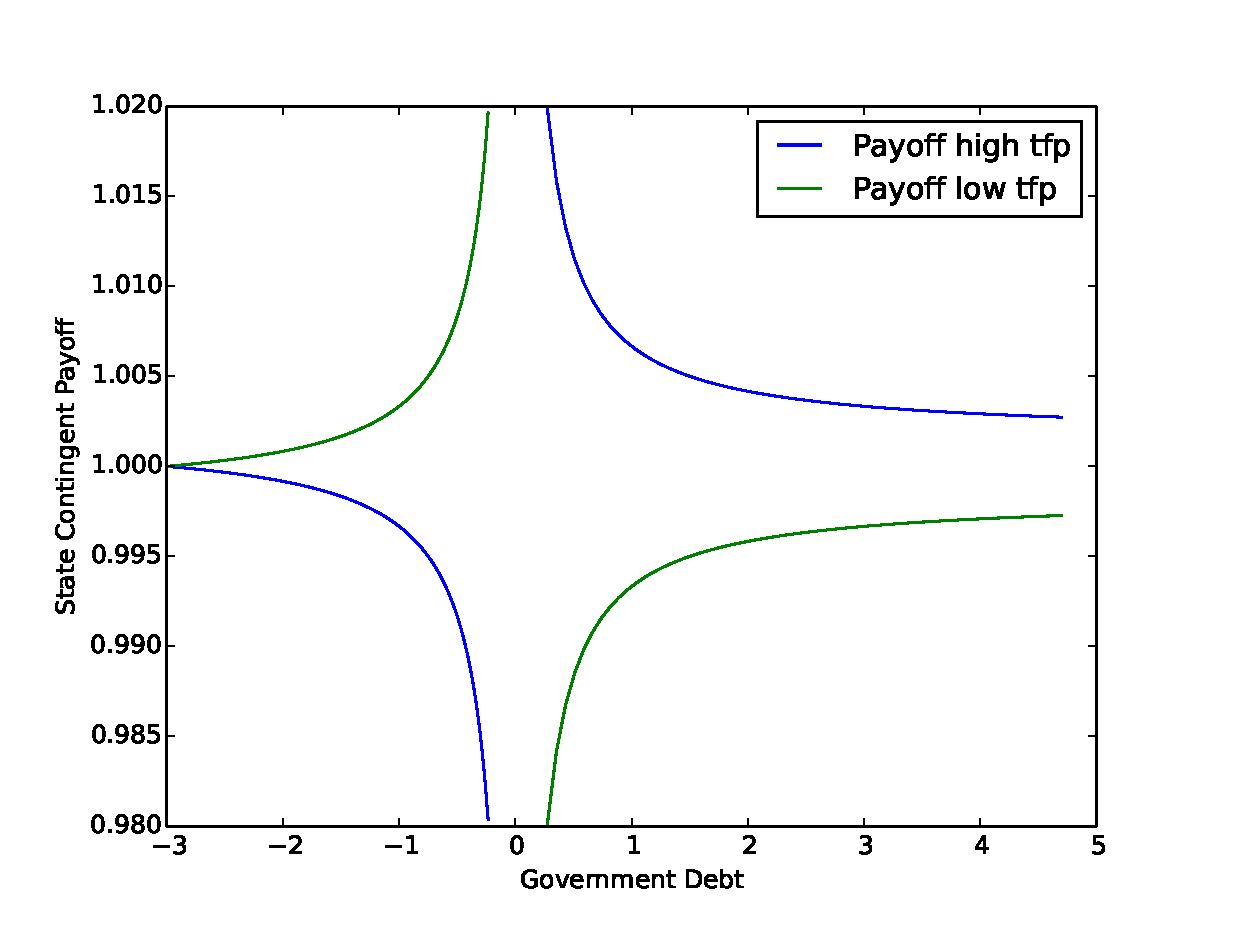
\includegraphics[scale=.4]{Images/p_graph_tfp.eps}
		\caption{Optimal asset payoff structure as a function of initial government debt when TFP follows a 2 shock i.i.d process}
	\end{center}	
	\end{figure}


\begin{figure}
		\begin{center}
		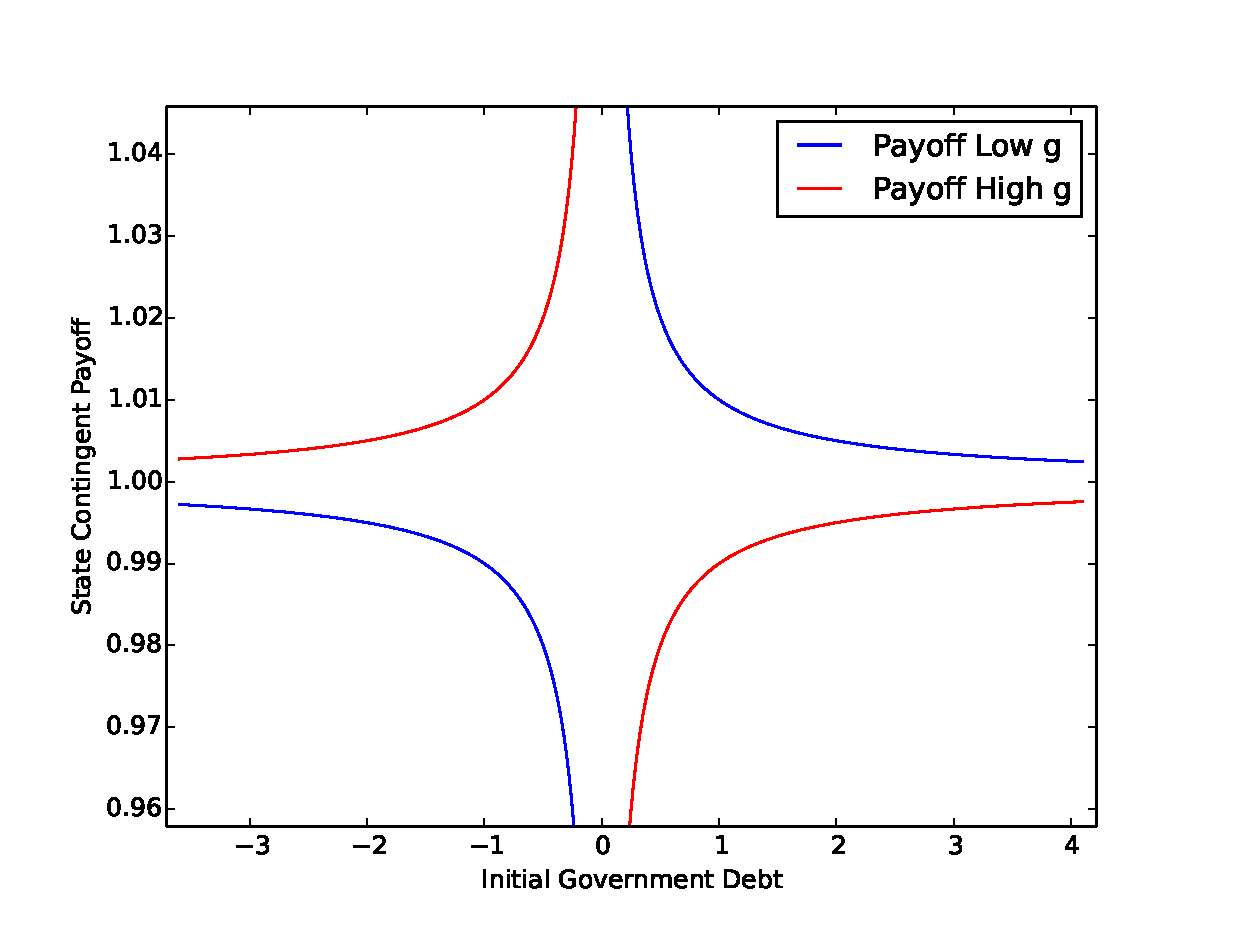
\includegraphics[scale=.4]{Images/p_graph.eps}
		\caption{Optimal asset payoff structure as a function of initial government debt when government expenditures follow 2 shock i.i.d process}
	\end{center}	
	\end{figure}


\subsection{Inverting the $\mathbb{P}^*$ mapping}
	\begin{enumerate}
		\item  \textbf{Exogenous payoff structure:} Suppose $\mathbb{P}\neq \mathbb{P}^*(b_{-1})$
		
		\item \textbf{Steady States: } A steady state is a government debt   $b^*$ such that
		\[b_{t}=b^* \text{ implies } b_{t+\tau}=b^*\quad \forall \tau >0\]
	
			
		\item \textbf{Characterization: } Given an asset payoff structure $\mathbb{P}$
		\begin{itemize}
			\item Does a steady state exist? Is it unique?
			\item Value of $b^*$?
			\item For what   \emph{initial government debts} $b_{-1}$ does  $b_t$ converge to $b^*$?
 			\end{itemize}
	\end{enumerate}

\subsection{Existence and $\mathbb{P}^{* -1}$}


 When shocks are i.i.d and take two values

  \begin{enumerate}

\item $\mathbb{P}(s\_,s)$ is independent of $s\_$ (so $\mathbb{P}$ can be a vector)
\item Under the normalization  $q_t = \beta$,  $\mathbb{E}\mathbb{P}(s)=1$.   Payoffs are then determined by a  scalar $\bm{p}$.
\begin{itemize}
 \item $\bm{p}$ is the asset's payoff in the ``good'' state $s$
 \item A risk-free bond is a security for which $\bm{p}=1$
\end{itemize}

\item A steady state is obtained by inverting the optimal payoff mapping $p^*$
\begin{equation*}
\label{eq-ss}
b^* \ \textrm{satisfies} \  \bm{p}=\bm{p}^*(b^*) \ \textrm{or} \ p^{* -1}(p) = b^*
\end{equation*}

One equation in one unknown $b^*$
\end{enumerate}

\subsection{Existence regions in $\bm{p}$ space}

The payoff $\bm{p}$ in good state
$\in (0,\infty)$.

We categorize a set of economies with different asset payoffs into 3 regions via thresholds $\alpha_2\geq\alpha_1\geq1$



  \begin{itemize}
   \item Low enough $\bm{p}(\leq \alpha_1$): government holds assets in steady state
   \item High enough $\bm{p} (\geq \alpha_2$): government  issues debt  in steady state
   \item Intermediate $\bm{p} (\alpha_1>\bm{p}>\alpha_2$): steady state does not exist
  \end{itemize}

\subsection{Thresholds: $\alpha_1 <\alpha_2$}
	%For either a pure TFP shock or a pure government expenditure shock,  we compute % $\alpha_1$ and $\alpha_2$ directly
	\begin{itemize}
		\item With only government expenditure shocks
		\[
			\alpha_1 = 1 \text{  and }  \alpha_2 = (1-\beta)\frac{\theta^\frac{\gamma}{1+\gamma}\left(\frac{1}{1+\gamma}\right)^\frac1\gamma\frac{\gamma}{1+\gamma}-g(s_1)}{\theta^\frac{\gamma}{1+\gamma}\left(\frac{1}{1+\gamma}\right)^\frac1\gamma\frac{\gamma}{1+\gamma}-\EE g} +\beta>1
		\]
		\item With only TFP shocks
		\[
			\alpha_1 = (1-\beta)\frac{\theta(s_1)^\frac{\gamma}{1+\gamma}}{\EE\theta^\frac{\gamma}{1+\gamma}}+\beta > 1
		\]and
		\[
		\alpha_2 = (1-\beta)\frac{\theta(s_1)^\frac{\gamma}{1+\gamma}\left(\frac{1}{1+\gamma}\right)^\frac1\gamma\frac{\gamma}{1+\gamma}-g}{\EE\theta^\frac{\gamma}{1+\gamma}\left(\frac{1}{1+\gamma}\right)^\frac1\gamma\frac{\gamma}{1+\gamma}-g}+\beta>\alpha_1
		\]
	\end{itemize}

	\begin{figure}
		\begin{center}
		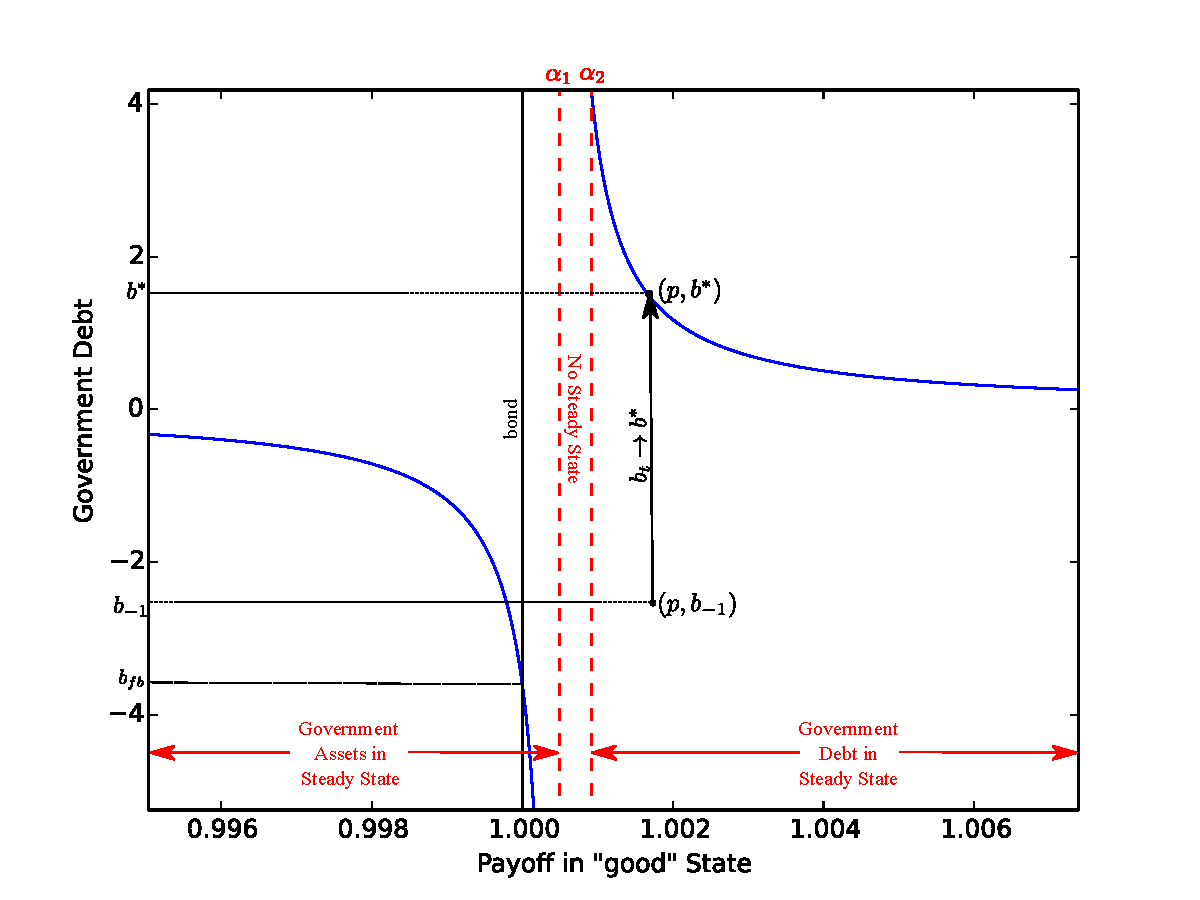
\includegraphics[width=4.2in]{Images/graph_nostable.pdf}
\caption{Existence regions in $\bm{p}$ space}
	\end{center}	
	\end{figure}

\subsection{Convergence}
  \begin{itemize}
		\item Our analysis verifies existence of a steady state in a 2-state i.i.d. economy.
		\item To study long-run properties of a Ramsey allocation, we want to know whether steady state is stable
		\item \textbf{Risk-adjusted martingale:}
		
		The Lagrange multiplier $\mu_t$ on the implementability  constraint   satisfies
		\[
			\mu_t = \EE_t p_{t+1} \mu_{t+1}
		\] or
		\[
		\EE_t  \mu_{t+1}	= \mu_t -Cov_t (p_{t+1}, \mu_{t+1})
		\]
			%\emph{$\mu_t$ follows a risk adjusted martingale.}
	
		\item \textbf{Stability criterion: }   Away from a steady state, is the drift  of $\mu_t$ big enough?
		\end{itemize}
	
\subsection{Characterizing convergence under quasi-linearity, iid, and $S=2$}

  \begin{itemize}
  \item Reminder:  $\bm{p}$ is the payoff in the ``good'' state.
   \item We partition  the ``$\bm{p}$ space'' into stable and unstable regions
     \end{itemize}

 	\begin{theorem}
Let $b^*$ denote steady state govt.  debt and $b_{fb}$ be  govt.  debt that  supports the first-best allocation with complete markets.  Then % for  same $  \alpha_1 < \alpha_2$
		\begin{enumerate}
			\item  \textbf{Low $\bm{p}$}: If $\bm{p}\leq\min(\alpha_1,1)$ then  $b_{fb}<b^*<0$ and $b_t\rightarrow b^*$ with probability 1.
			\item \textbf{High  $\bm{p}$}:  If $\bm{p} \geq \alpha_2$ then   $0<b^*$ and $b_t \rightarrow b^*$ with probability 1.
			
			
			\end{enumerate}
			\end{theorem}
			
			For the intermediate region where  $b^*$ either does not exist or is unstable, there is a tendency to run up debt


{Stability regions}
	\begin{figure}
		\begin{center}
		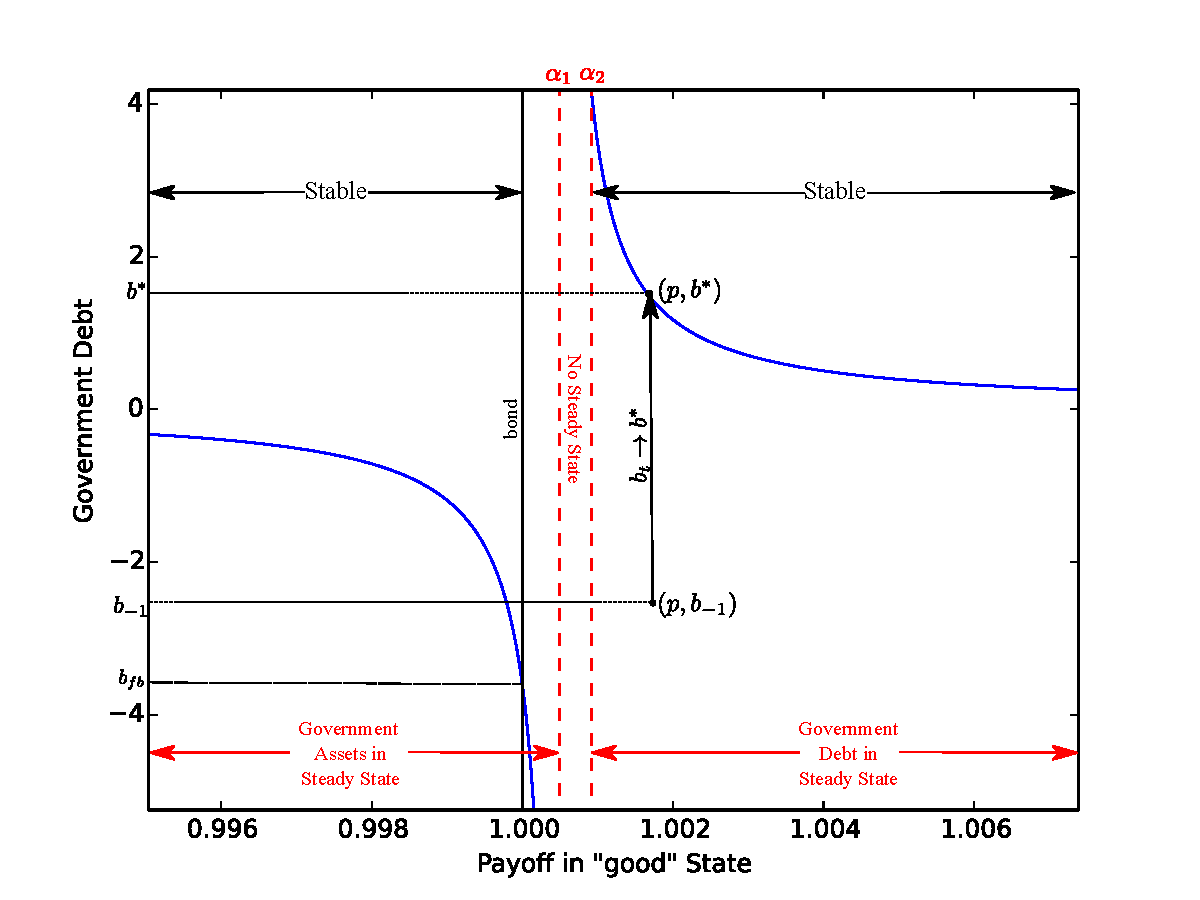
\includegraphics[width = 4.2in]{Images/graph_stable.pdf}
\caption{Stability regions}
	\end{center}	
	\end{figure}	

\begin{figure}
	\begin{center}
	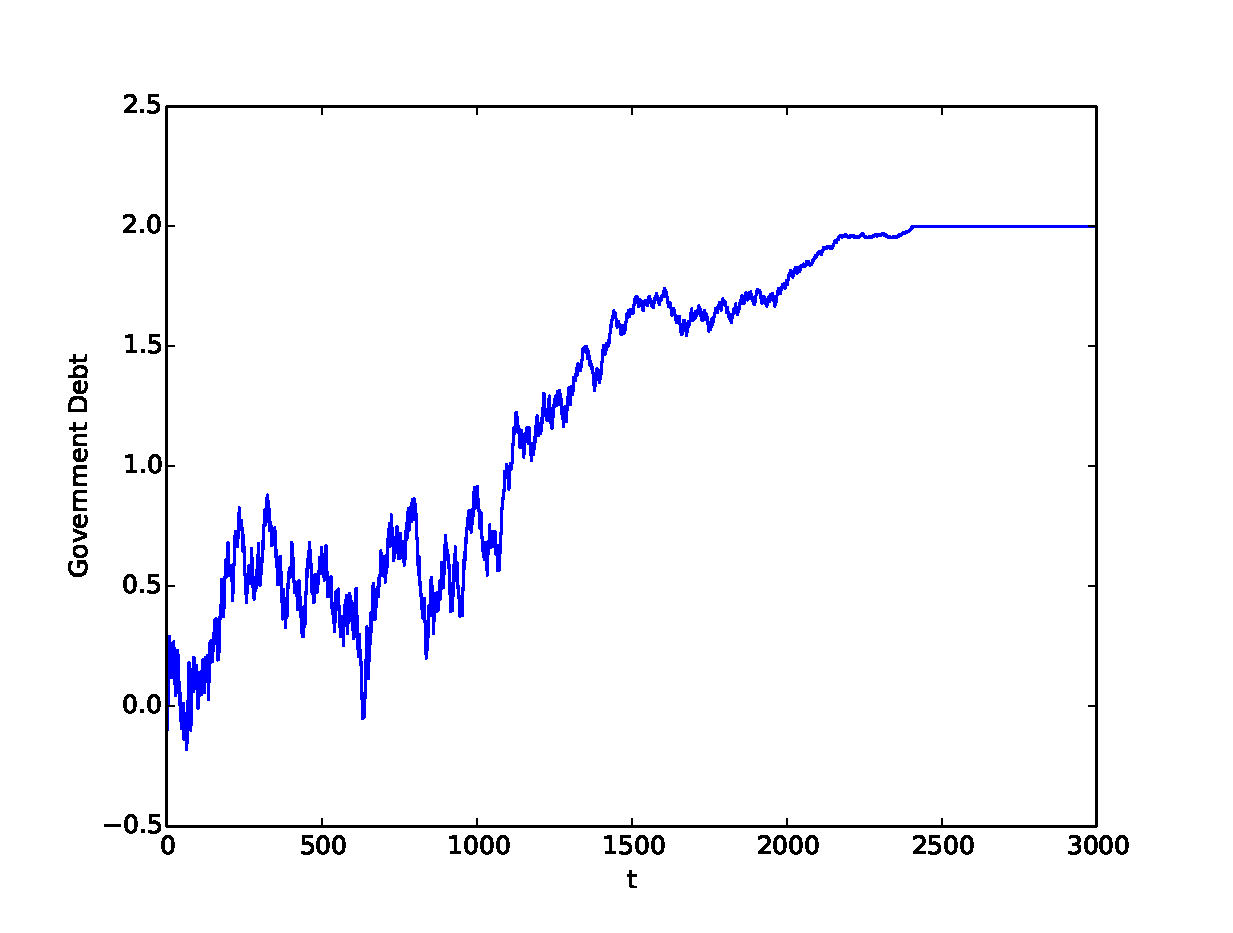
\includegraphics[width=4in]{Images/port1.eps}
    \caption{A sample path with  $\bm{p} > 1$}
	\end{center}
\end{figure}

\begin{figure}
	\begin{center}
	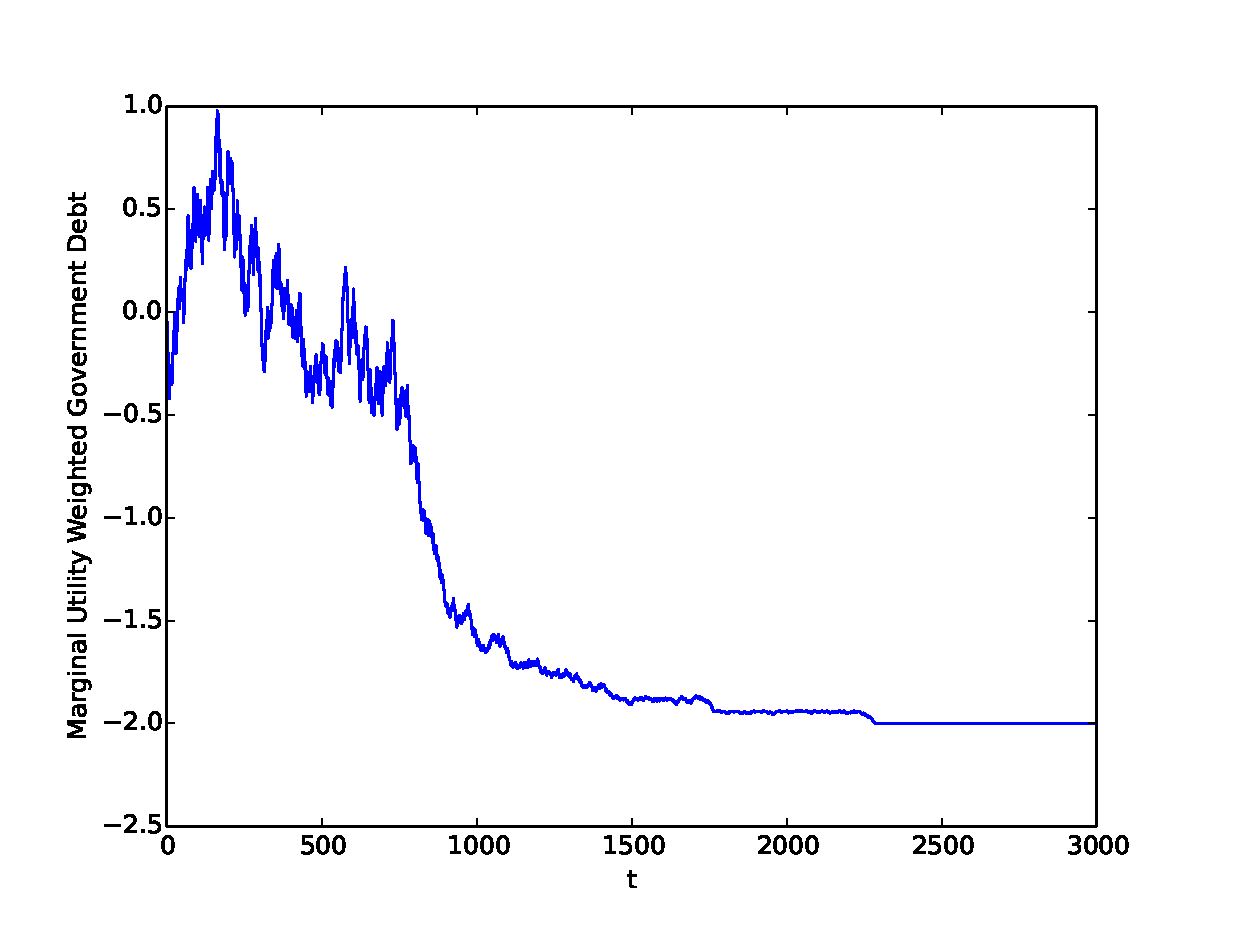
\includegraphics[width=4in]{Images/port2.eps}
\caption{A sample path with   $\bm{p} <1$}
	\end{center}	
\end{figure}

\subsection{Intuition for Convergence}
	\small
	\begin{itemize}
	%\begin{itemize}
	%\item Debt {\color{black} \textbf{levels} } can help smooth tax distortions {\color{black}\textbf{across  states}}
	%\item This differs from the  role of debt economies with risk free debt where {\color{black} \textbf{changes}} in debt levels help smooth tax distortions {\color{black}  \textbf{over  time}}
	%\end{itemize}
	\item The Ramsey policy with incomplete markets smooths the welfare costs of distorting labor taxes by manipulating debt positions
	\item With a risk-free bond, the marginal cost of raising funds $\mu_t$ is  a martingale. Changes in debt levels help smooth tax distortions across time. 		
	\item  If the payoff matrix of the asset differs across states, then  by generating state contingent revenues, the level of government debt smooths tax distortions across states.
	\item The steady state $b^*$ is a unique debt level that provides enough ``state contingency'' completely to overcome  missing assets markets	
	\item  When issuing debt, the government takes takes this benefit into account by distorting the martingale and either accumulating or decumulating debt.	
	\item Although this is achieved by raising taxes, locally  the welfare costs of taxes are second order and dominated by the gains from coming closer to $b^*$, which are first order in terms of welfare.
	%\item This explains the long run convergence to $b^*$
	\end{itemize}


\subsection{Outcomes with quasi-linear preferences}
 \textbf{Outcomes:}
 \begin{enumerate}
  \item  Often $b_t\to b^*$ when the aggregate state follows a 2-state i.i.d. process
  \item The level  and sign of $b^*$ depend on the \textbf{exogenous payoff structure} $\mathbb{P}$
  \item The limiting allocation corresponds to a complete market Ramsey allocation for initial govt. debt $b^*$
 \end{enumerate}
 
 
 \subsection{Turning on risk-aversion}
  \textbf{Modifications:}
  \begin{itemize}
  \item Another source of return fluctuations -- the risk-free interest rate
   \item Marginal utility adjusted debt  encodes history dependence
   \item  With binary i.i.d shock shock process,  $x_t=u_{c,t}b_{t}$  converges

   \item Long-run properties of $x_t$ depend on equilibrium returns $R_{t,t+1}=\frac{\mathbb{P}(s_t,s_{t+1})}{q_t(s^t)}$.
   Now $q_t$ varies in interesting ways


  \end{itemize}
  
  
  
\subsection{Roadmap, II}


 Two subproblems
\begin{enumerate}
 \item  $t=0$ Bellman equation in value function $W(b_{-1},s_0)$ %\textcolor{red}{Anmol and David XXXXXX: I altered the notation}
 \item  $t\geq 1$ Bellman equation in value function $V(x,s\_)$
\end{enumerate}

Seek steady states $x^*$ such that $x_t \to x^*$

\subsection{A Recursive Formulation}
	
	\begin{enumerate}
	 \item Commitment implies that government actions at $t \geq 1$ are constrained by the public's anticipations about them at $s < t$
	 \item This contributes additional state variables like marginal utility of consumption
	 \item Scaling the budget constraint by marginal utility makes Ramsey problem  recursive in  $x=U_c b$
	
	\[
		\frac{x_{t-1} p_t U_{c,t}}{\beta \EE_{t-1} p_t U_{c,t}}  = U_{c,t}c_t+U_{l,t} l_t + x_t
	\]
	
	%\item The planner's problem recursively with a single state variable.
	\end{enumerate}
	
	
	\subsection{Bellman equation for $t\geq1$ (\textit{ex ante})}
	\[
		V(x,s\_) = \max_{c(s),l(s),x'(s)} \sum_s \Pi(s,s\_)\Bigl(U(c(s),l(s)) + \beta V(x'(s),s)\Bigr)
	\]subject to $x'(s)\in [\underline x,\overline x]$
	\begin{align*}
		\frac{x \mathbb{P}(s) U_c(s)}{\beta\EE_{s\_} \mathbb{P}Uc} =U_c(s)c(s)+U_l(s)l(s) + x'(s)\\
		c(s) + g(s) = \theta(s)l(s)
	\end{align*}
	
 \subsection{Time $0$ Bellman equation (\textit{ex post})}
	Given an initial  debt $b_{-1}$, state $s_0$,  and continuation value function $V(x,s\_)$
%\textcolor{red}{Anmol and David XXXXX: I altered the below by adding the $W$ function; but there is a problem with the timing of
%the $b$ argument.  See earlier slide where $W$ is defined.}
	\[
		W(b_{-1},s_0) = \max_{c_{0},l_0,x_{0}} U(c,l) +\beta V(x_0,s0)
	\]subject to  time zero implementability constraint
	\[
		U_{c}(c_0,l_0)c + U_l(c_0,l_0) l_0 + x_0 = U_c(c_0,l_0) b_{-1}
	\]and  resource constraint
	\[
		c_0+ g(s_0) = \theta(s_0) l_0
	\]and
	\[
		x_0 \in [\underline x,\overline x]
	\]


\end{document}
